\section{Performance Evaluation}
\label{results}
This section evaluates the performance of the traffic analysis methodology introduced in Section~\ref{sec:methodology}. We assess the effectiveness of the XGBoost-based classifier for the two traffic analysis tasks considered in this work—device type classification and individual device identification—under both intra-topology and cross-topology evaluation settings.

The evaluation is structured as follows. First, we perform a preliminary analysis to identify the optimal temporal window size for feature extraction. We then report classification performance when training and testing are conducted within the same network topology, representing the standard evaluation scenario adopted in the literature. Finally, we analyze the generalization capability of the model by evaluating performance across different network topologies.


\subsection{Optimal Time Window Selection}



\begin{figure}[htbp]
    \centering

    \begin{subfigure}[b]{0.504\linewidth}
        \centering
        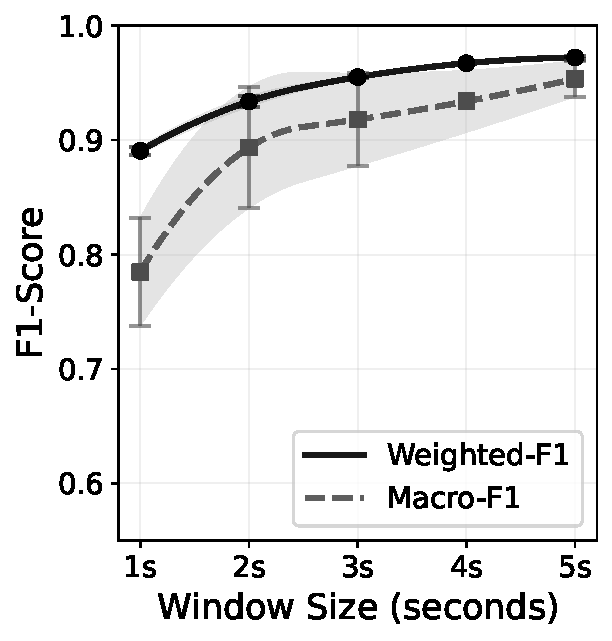
\includegraphics[width=\linewidth,trim={8 8 7 7},clip]{Figures/time-window/figure1_device_type.pdf}
        \caption{Device Type Classification}
        \label{fig:device_type_classification}
    \end{subfigure}
    \hfill
    \begin{subfigure}[b]{0.425\linewidth}
        \centering
        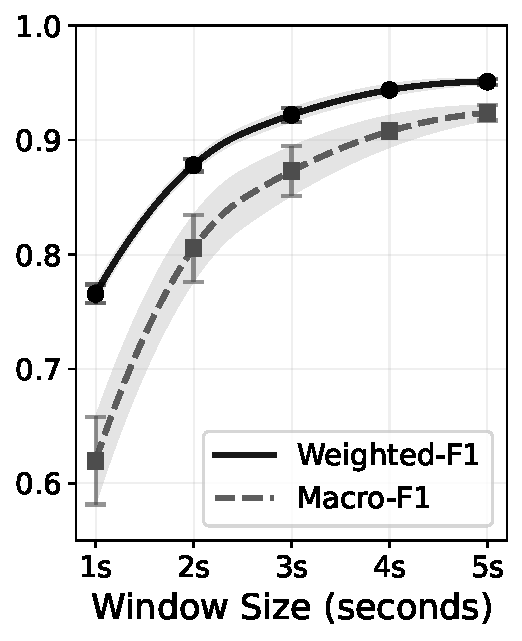
\includegraphics[width=\linewidth,trim={8 8 6 7},clip]{Figures/time-window/figure2_device_name.pdf}
        \caption{Individual Device Identification}
        \label{fig:device_name_classification}
    \end{subfigure}
\caption{Weighted and Macro F1-Score across different window sizes for: (a) device type classification and (b) individual device identification classification task.} 
\label{fig:f1_score_comparison} 
\end{figure}


Before proceeding with the main classification experiments, we conducted a preliminary study to determine the optimal temporal window size for feature extraction. Since our approach aggregates network traffic data using time windows, this parameter critically affects the trade-off between capturing sufficient temporal context and maintaining adequate sample sizes for robust classification.
We tested five different window lengths (1, 2, 3, 4, and 5 seconds), training and evaluating the XGBoost classifier for each configuration. Figure \ref{fig:f1_score_comparison} presents the weighted and macro F1-scores across these window sizes, revealing a consistent trend for both tasks: classification performance improves steadily with increasing window size, as longer windows more effectively capture meaningful temporal patterns in network traffic data.
Specifically, for device type classification, the weighted F1-score increased from 0.89 (1-second window) to 0.97 (5-second window), and the macro F1-score improved from 0.78 to 0.95. For individual device identification, in the same range of window sizes, the weighted F1-score increased from 0.76 to 0.95, and the macro F1-score from 0.62 to 0.92.
Both tasks exhibit performance curves approximating a saturating exponential function, characterized by rapid initial gains followed by progressively diminishing returns. The marginal improvement beyond the 4-second threshold is minimal, suggesting that a 5-second window captures nearly all relevant temporal dynamics. Based on this empirical characterization and considering the trade-off between classification performance, computational efficiency, and prediction time, we fixed the sliding window size at 5 seconds for all subsequent experiments presented in the next sections.

Before presenting the classification results, a statistical analysis of the ML-ready dataset (described in Section \ref{sec:data_pre}) revealed that \gls*{redfd} devices, which typically transmit single Zigbee packets in response to specific events, can produce windows containing insufficient packets (i.e., windows with fewer than 2 packets) for meaningful feature extraction. Consequently, two devices: the Sonoff temperature sensor and the Aquara Vibration sensor, yielded fewer than 10 valid 5-second windows across both topologies and were excluded from further analysis.

Based on these results, a 5-second temporal window was selected for all subsequent experiments.

\subsection{Intra-topology Classification}
We first evaluate classification performance under an intra-topology setting, where training and testing data originate from the same Zigbee network topology. This scenario represents the standard evaluation setup adopted in prior work on IoT traffic classification and serves as a baseline for subsequent cross-topology analysis. All results are obtained using stratified 5-fold cross-validation.

\subsubsection{Device Type Classification}
The proposed classifier achieves excellent performance when evaluated under the intra-topology setting. Using a 5-second temporal window and topology~B, the model attains a weighted F1-score of 0.97 and a macro F1-score of 0.95. The corresponding classification report and normalized confusion matrix are shown in Table~\ref{tab:cls-type_topo_B} and Figure~\ref{fig:cls-type_topo_B}, respectively.

High precision and recall are consistently observed across nearly all device categories, indicating strong discriminative capability between different smart home device types. Comparable results are obtained for topology~A, as summarized in Table~\ref{tab:classification_results_type}.


\begin{figure}[t]
\centering
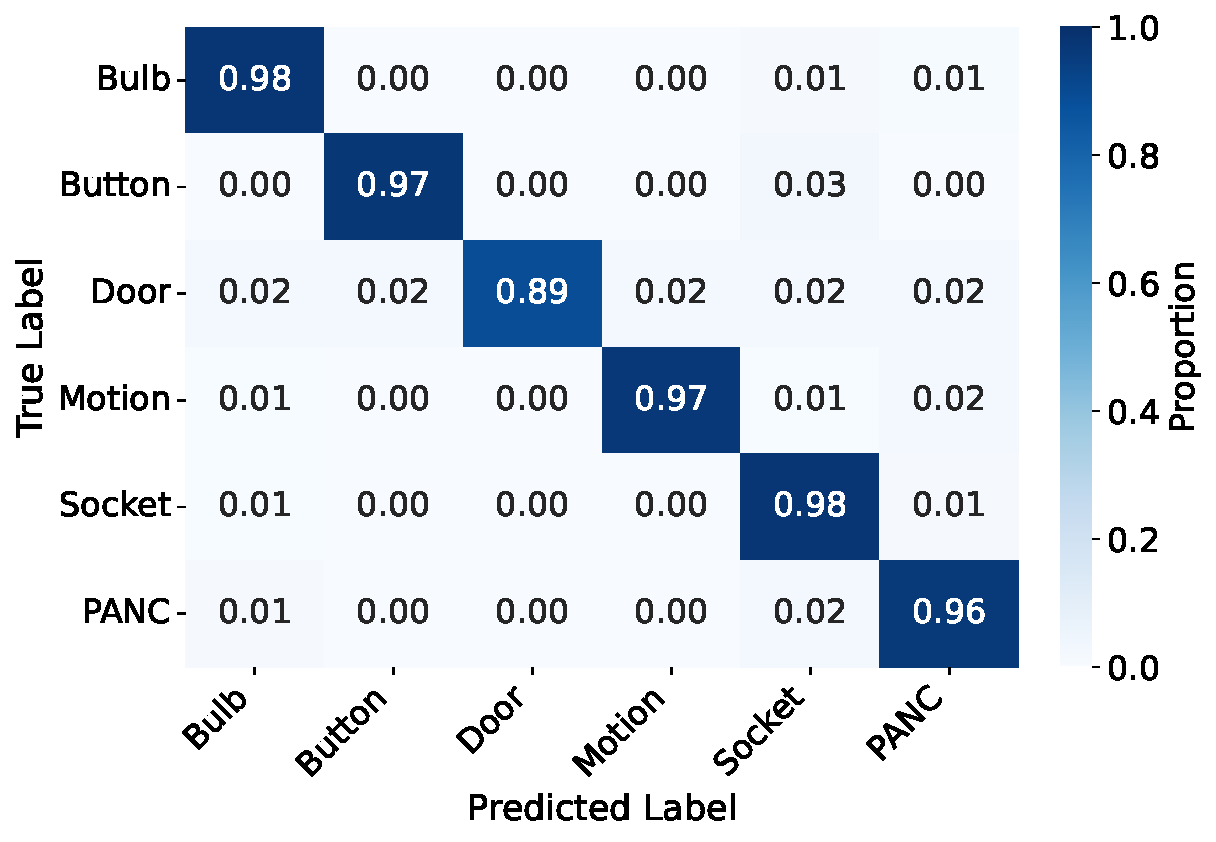
\includegraphics[width=0.7\linewidth]{Figures/confusion_matrix/confusion_matrix_relative_device_type_topoB.pdf}
\caption{Normalized Confusion matrix for device type classification on a 5-second window in topology B.}
\label{fig:cls-type_topo_B}
\end{figure}

\begin{table}[htbp]
    \centering
    \begin{tabular}{lccc}
    \toprule
    \textbf{Class} & \textbf{Precision} & \textbf{Recall} & \textbf{F1-score} \\
    \midrule
    Bulb         & 0.94 & 0.98 & 0.96  \\
    Button       & 0.92 & 0.97 & 0.95 \\
    Coordinator  & 0.98 & 0.96 & 0.97 \\
    Door         & 0.98 & 0.89 & 0.93 \\
    Motion       & 0.92 & 0.97 & 0.94 \\
    Socket       & 0.98 & 0.98 & 0.98 \\
    \midrule
    \textbf{Accuracy}     &       &       & 0.97 \\
    \textbf{Macro Avg}    & 0.95 & 0.96 & 0.95  \\
    \textbf{Weighted Avg} & 0.97 & 0.97 & 0.97 \\
    \bottomrule
    \end{tabular}
    \caption{Classification report for device type classification on a 5-second window in topology B.}
    \label{tab:cls-type_topo_B}
\end{table}


\subsubsection{Individual Device Identification}
Despite the increased complexity of individual device identification, the classifier maintains strong performance under the intra-topology setting. With 14 distinct device identities, the model achieves a weighted F1-score of 0.95 and a macro F1-score of 0.93 when evaluated on topology~B.

The normalized confusion matrix and classification report, shown in Figure~\ref{fig:cls-name_topo_B} and Table~\ref{tab:device_name_classification_topoB}, respectively, indicate robust performance across most devices. The \gls*{panc} is particularly well distinguished, likely due to its unique role in network coordination. Results for both topology~A and B are reported in Table~\ref{tab:classification_results_name}.


\begin{figure*}[htbp]
\centering
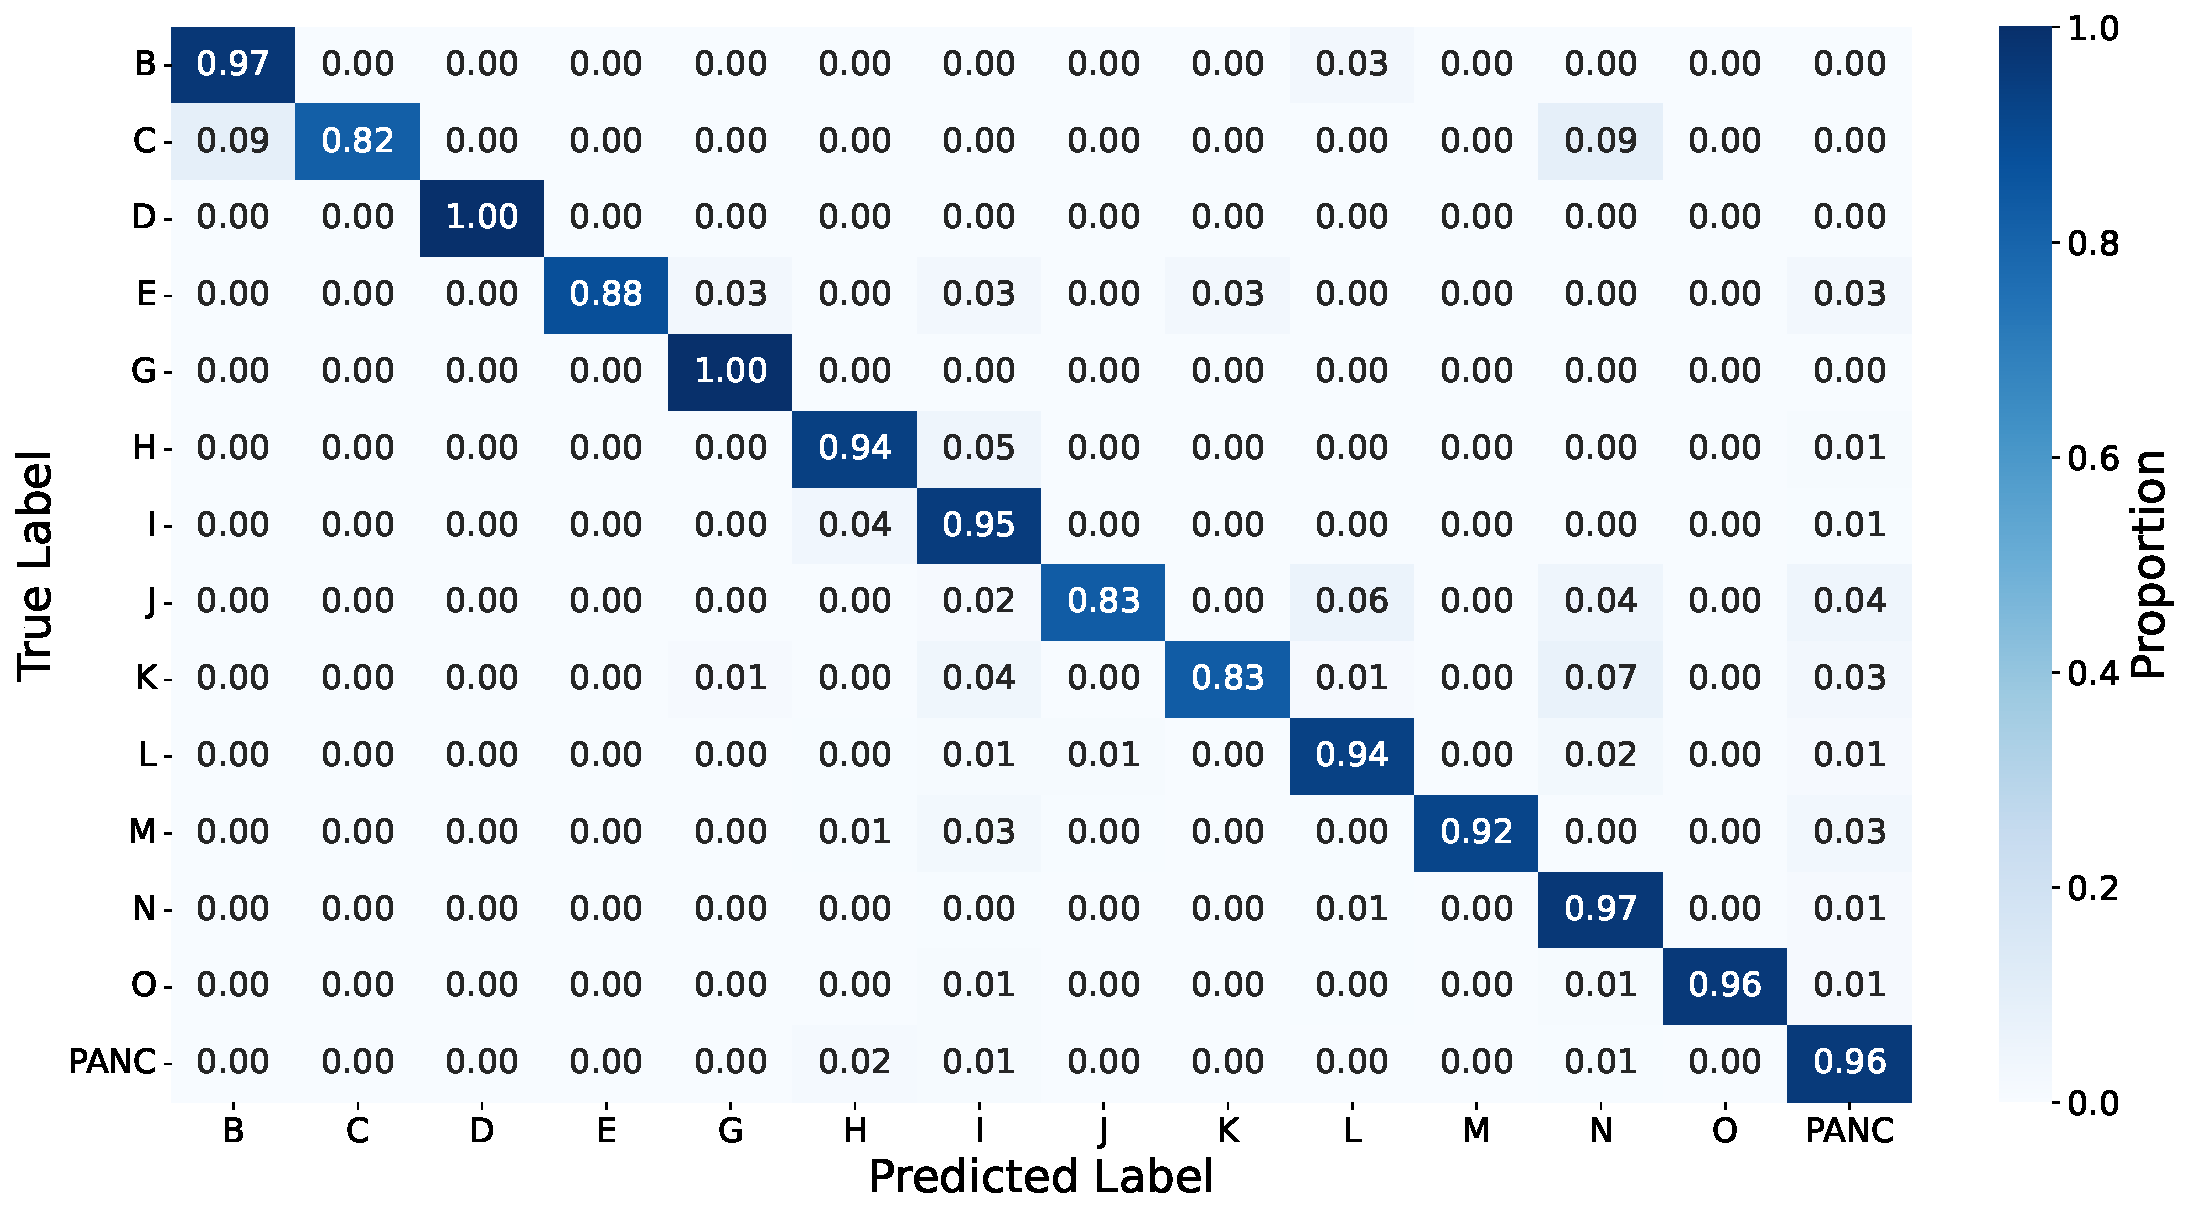
\includegraphics[width=0.9\linewidth]{Figures/confusion_matrix/confusion_matrix_relative_device_name_topoB.pdf}
\caption{Normalized Confusion matrix for individual device identification on a 5-second window in topology B.}
\label{fig:cls-name_topo_B}
\end{figure*}

\begin{table}[t]
    \centering
    \begin{tabular}{llccc}
    \toprule
    \textbf{Class} & \textbf{Class Name} & \textbf{Precision} & \textbf{Recall} & \textbf{F1-score} \\
    \midrule
  B & Sonoff Motion Sensor  & 0.84 & 0.97 & 0.90 \\
  C & Sonoff Door Sensor & 0.90 & 0.82 & 0.86 \\
  D & Aqara Motion Sensor & 1.00 & 1.00 & 1.00 \\
  E & Aqara Door/Window Sensor & 1.00 & 0.88 & 0.94 \\
  G & Aqara Mini Switch & 0.92 & 1.00 & 0.96 \\
  H & Tuya Smart Socket & 0.91 & 0.94 & 0.92 \\
  I & Senckit Smart Power Plug & 0.95 & 0.95 & 0.95 \\
  J & Ledvance Z3 Plug & 0.87 & 0.83 & 0.85 \\
  K & Ledvance Smart+ Plug  & 0.88 & 0.83 & 0.85 \\
  L & Ledvance Smart+ Bulb  & 0.94 & 0.94 & 0.94 \\
  M & Moes Bulb & 0.95 & 0.92 & 0.94 \\
  N & Philips HueLamp  & 0.93 & 0.97 & 0.95 \\
  O & Philips HueMotion  & 0.92 & 0.96 & 0.94 \\ 
  PANC &Pan Coordinator & 0.98 & 0.96 & 0.97 \\
  % B & 0.84 & 0.97 & 0.90 \\
  % C & 0.90 & 0.82 & 0.86 \\
  % D & 1.00 & 1.00 & 1.00 \\
  % E & 1.00 & 0.88 & 0.94 \\
  % G & 0.92 & 1.00 & 0.96 \\
  % H & 0.91 & 0.94 & 0.92 \\
  % I & 0.95 & 0.95 & 0.95 \\
  % J & 0.87 & 0.83 & 0.85 \\
  % K & 0.88 & 0.83 & 0.85 \\
  % L & 0.94 & 0.94 & 0.94 \\
  % M & 0.95 & 0.92 & 0.94 \\
  % N & 0.93 & 0.97 & 0.95 \\
  % O & 0.92 & 0.96 & 0.94 \\ 
  % PANC & 0.98 & 0.96 & 0.97 \\
    \midrule
    \textbf{Accuracy}     &&       &       & 0.95 \\
    \textbf{Macro Avg}    && 0.93 & 0.93 & 0.93  \\
    \textbf{Weighted Avg} && 0.95 & 0.95 & 0.95 \\
    \bottomrule
    \end{tabular}
    \caption{Classification report for individual device identification using a 5-second temporal window in topology B.}
    \label{tab:device_name_classification_topoB}
\end{table}


\begin{table}[t]
\centering
\footnotesize
\setlength{\tabcolsep}{3.5pt}
\renewcommand{\arraystretch}{1.1}
\caption{Classification Results Summary for Device Type classification task}
\label{tab:classification_results_type}
\begin{tabularx}{\columnwidth}{l l c c c c c}
\toprule
\textbf{Train} & \textbf{Test} & \textbf{Accuracy} & \textbf{Precision} & \textbf{Recall} & \textbf{F1-Macro} & \textbf{F1-Weighted} \\
\textbf{Dataset} & \textbf{Dataset} &  &  &  &  &  \\
\midrule
\multicolumn{7}{c}{\textbf{Intra-Topology (K-Fold, k=5)}} \\
\midrule
Topo. A & Topo. A & 0.970 $\pm$ 0.003 & 0.949 $\pm$ 0.013 & 0.944 $\pm$ 0.022 & 0.945 $\pm$ 0.010 & 0.971 $\pm$ 0.003 \\
Topo. B & Topo. B & 0.972 $\pm$ 0.002 & 0.953 $\pm$ 0.018 & 0.957 $\pm$ 0.013 & 0.954 $\pm$ 0.016 & 0.972 $\pm$ 0.002 \\
\midrule
\multicolumn{7}{c}{\textbf{Cross-Topology (Full Dataset)}} \\
\midrule
Topo. A & Topo. B & 0.878 & 0.738 & 0.765 & 0.745 & 0.879 \\
Topo. B & Topo. A & 0.850 & 0.724 & 0.759 & 0.741 & 0.849 \\
\bottomrule
\end{tabularx}
\end{table}




% \begin{table}[]
% \centering
% \caption{Classification Results Summary for Device Type classification task}
% \label{tab:classification_results_type}
% \begin{tabular}{\columnwidth}{|l|l|c|c|c|c|c|}
% \hline
% \textbf{Training} & \textbf{Test} &  \textbf{Accuracy} & \textbf{Precision} & \textbf{Recall} & \textbf{F1-Macro} & \textbf{F1-Weighted}  \\
% \textbf{Dataset} & \textbf{Dataset} & & & & & \\
% \hline
% \multicolumn{7}{|c|}{\textbf{Intra-Topology (K-Fold, k=5)}} \\
% \hline
%  Topology A & Topology A  & 0.970 ± 0.003  & 0.949 ± 0.013 & 0.944 ± 0.022 & 0.945 ± 0.010 & 0.971 ± 0.003 \\
% \hline
%  Topology B & Topology B  & 0.972 ± 0.002  & 0.953 ± 0.018 & 0.957 ± 0.013 & 0.954 ± 0.016 & 0.972 ± 0.002 \\
% \hline
% \multicolumn{7}{|c|}{\textbf{Cross-Topology (Full Dataset)}} \\
% \hline
% Topology A & Topology B  & 0.878 & 0.738 & 0.765 & 0.745 & 0.879 \\
% \hline
%  Topology B & Topology A  & 0.850 & 0.724 & 0.759 & 0.741 & 0.849 \\
% \hline
% \end{tabular}
% \end{table}



% \begin{table*}[]
% \centering
% \caption{Classification Results Summary for individual device identification task}
% \label{tab:classification_results_name}
% \begin{tabular}{|l|l|c|c|c|c|c|}
% \hline
% \textbf{Training} & \textbf{Test} &  \textbf{Accuracy} & \textbf{Precision} & \textbf{Recall} & \textbf{F1-Macro} & \textbf{F1-Weighted}  \\
% \textbf{Dataset} & \textbf{Dataset} & & & & & \\
% \hline
% \multicolumn{7}{|c|}{\textbf{Intra-Topology (K-Fold, k=5)}} \\
% \hline
%   Topology A & Topology A  & 0.944 ± 0.004  & 0.910 ± 0.032 & 0.877 ± 0.017 & 0.889 ± 0.021 & 0.944 ± 0.004 \\
% \hline
%   Topology B & Topology B  & 0.951 ± 0.003  & 0.932 ± 0.016 & 0.924 ± 0.019 & 0.923 ± 0.007 & 0.951 ± 0.003 \\
% \hline
% \multicolumn{7}{|c|}{\textbf{Cross-Topology (Full Dataset)}} \\
% \hline
% Topology A & Topology B & 0.692 & 0.517 & 0.480 & 0.474 & 0.694 \\
% \hline
%  Topology B & Topology A  & 0.678 & 0.446 & 0.434 & 0.413 & 0.672 \\
% \hline
% \end{tabular}
% \end{table*}

\begin{table}[t]
\centering
\footnotesize
\setlength{\tabcolsep}{3pt}
\renewcommand{\arraystretch}{1.1}
\caption{Classification Results Summary for individual device identification task}
\label{tab:classification_results_name}
\begin{tabular}{llccccc}
\toprule
\textbf{Train} & \textbf{Test} & \textbf{Accuracy} & \textbf{Precision} & \textbf{Recall} & \textbf{F1-Macro} & \textbf{F1-Weighted} \\
\textbf{Dataset} & \textbf{Dataset} &  &  &  &  &  \\
Topo. A & Topo. A & 0.944 $\pm$ 0.004 & 0.910 $\pm$ 0.032 & 0.877 $\pm$ 0.017 & 0.889 $\pm$ 0.021 & 0.944 $\pm$ 0.004 \\
Topo. B & Topo. B & 0.951 $\pm$ 0.003 & 0.932 $\pm$ 0.016 & 0.924 $\pm$ 0.019 & 0.923 $\pm$ 0.007 & 0.951 $\pm$ 0.003 \\
\midrule
\multicolumn{7}{c}{\textbf{Cross-Topology (Full Dataset)}} \\
\midrule
Topo. A & Topo. B & 0.692 & 0.517 & 0.480 & 0.474 & 0.694 \\
Topo. B & Topo. A & 0.678 & 0.446 & 0.434 & 0.413 & 0.672 \\
\bottomrule
\end{tabular}
\end{table}




\subsection{Cross-topology Classification}
We next evaluate the generalization capability of the proposed traffic analysis methodology by adopting a cross-topology setting, in which training and testing are performed on data collected from different Zigbee network topologies. This evaluation exploits the multi-topology nature of the dataset and allows us to quantify the impact of topology-dependent traffic dynamics on classification performance.


\subsubsection{Device Type Classification}
Device type classification exhibits moderate performance degradation under cross-topology evaluation. When trained on one topology and tested on the other, the model achieves a weighted F1-score of approximately 0.85 and a macro F1-score of 0.75 (Table~\ref{tab:classification_results_type}).

While the \gls*{panc} remains consistently well classified, device categories dominated by \glspl*{redfd} experience larger performance drops. This behavior is attributable to limited training support and to topology-dependent routing effects introduced by the Zigbee mesh network. Overall, the classifier remains effective at distinguishing device types, reflecting the standardized command sets and communication patterns enforced by the Zigbee protocol.


\begin{figure}[t]
    \centering
    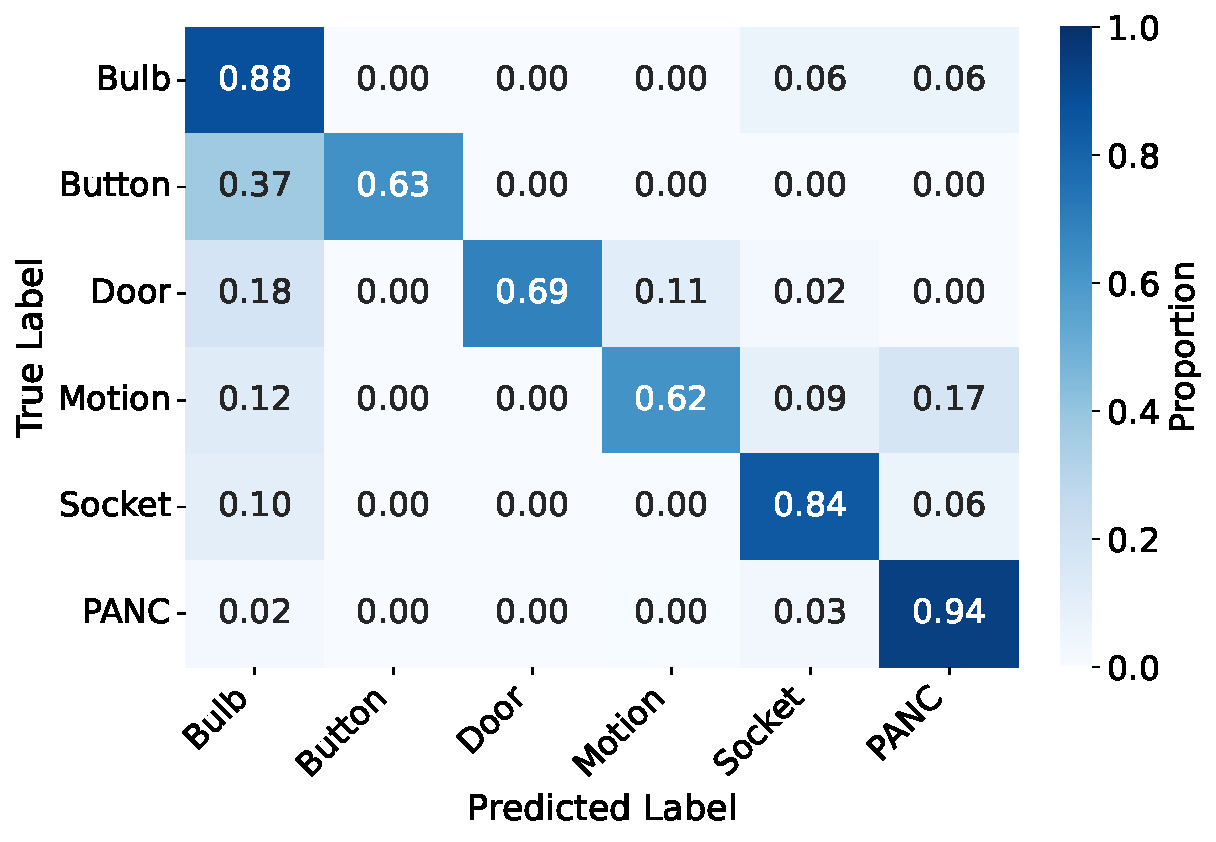
\includegraphics[width=0.7\linewidth]{Figures/confusion_matrix/confusion_matrix_relative_device_type_topo_trainAoverB.pdf}
    \caption{Normalized Confusion matrix for device type classification on cross-topology settings (trained on network traces acquired from topology B and tested against network traces coming from topology A.}
    \label{fig:cross-topo-cm}
\end{figure}
\subsubsection{Individual Device Identification}
In contrast, individual device identification is strongly affected by topology changes. When trained on topology~B and tested on topology~A, accuracy drops to 0.68, with a weighted F1-score of 0.67 and a macro F1-score of 0.41 (Table~\ref{tab:classification_results_name}).

The most significant degradation is observed for \glspl*{redfd}, whose average per-device F1-score falls below 0.2. This effect is exacerbated by the fine-grained nature of the task, which increases the number of classes and reduces the number of training samples per class. \glspl*{ffd} demonstrate comparatively higher robustness, with an average F1-score of 0.53, while the \gls*{panc} maintains stable performance (F1-score of 0.86), indicating largely topology-invariant traffic patterns.

Misclassifications predominantly occur among devices of the same manufacturer or device category, suggesting that manufacturer-specific traffic characteristics exhibit partial resilience to topology changes, whereas device-specific fingerprints are more sensitive to mesh routing dynamics.

\subsection{Discussion}
The experimental results highlight the effectiveness and the limitations of traffic-based device profiling in Zigbee networks. Under intra-topology conditions, the proposed methodology achieves excellent performance for both device type classification and individual device identification, confirming that encrypted Zigbee traffic retains sufficient behavioral information to support fine-grained analysis.

However, the cross-topology evaluation reveals a markedly different behavior between the two tasks. While device type classification shows only moderate performance degradation, individual device identification is significantly affected by changes in network topology. This divergence can be attributed to the standardized nature of Zigbee application profiles, which enforces consistent communication patterns at the device category level, in contrast to device-specific characteristics that are more sensitive to mesh routing dynamics and multi-hop communication paths.

The observed degradation is particularly pronounced for battery-powered \glspl*{redfd}, whose sparse and event-driven traffic, combined with relay operations performed by \glspl*{ffd}, reduces the stability of temporal traffic features across topologies. Conversely, mains-powered devices and the \gls*{panc} exhibit more robust and topology-invariant traffic patterns, resulting in higher classification resilience.

